\section{질문, 범위와 계산 결과}
\subsection{고정한 물리 계열}
이번 질문은 HH source 강도 $\lambda$와 photon birth 진폭 $b$가
한 구간의 온도 결함 $F$를 각각 얼마나 휘게 만드는가이다.
PHYS18의 허용 계수 선택 $\alpha$ 하나를 고정하고,
같은 COMMON과 모든 단계에 공통인 $(\lambda,b)\in[0,1]^2$를 사용했다.
각 $\alpha$의 실제 계열에 대해 도함수를 취하고, 포함은 그 허용 계열 전체에 균일하다.
원 source에 맞춘 geometric-isotropic $C^2$ closure, gas 영역과 연결 선분,
양의 분모 및 검증된 implicit root branch를 그대로 사용한다.
경계 도함수에는 계약의 열린 근방을 사용한다.

상태와 시간 길이는
\[
g=(x_{\rm HII},y_{\rm HeII},y_{\rm HeIII},w_{\rm eV/H}),\qquad
h=625000000\ {\rm s},\quad \Delta t_F=2h
\]
이며, $t_0=160000000000\ {\rm s}$,
$t_1=160625000000\ {\rm s}$,
$t_2=161250000000\ {\rm s}$이다.
33개 활성 photon node와 number·energy guard 두 개를 모두 보존했다.
원 native leaves의 $c,\chi_H,k_B,\epsilon_{\rm eV}$를 사용하며,
밀도비는 저장된 두 밀도의 정확한 비
$f=\operatorname{exact}(n_{\rm He})/\operatorname{exact}(n_H)$다.
이 축소 source 계산에서 새 spacetime metric convention을 도입하지 않는다.

이 보고서에서 $F$와 그 매개변수 응답은 \emph{정의된 두 이산 경로 사이의 차이}다.
그 차이를 동일 물리 계열에서 정량적으로 해석하는 것이 이번 성과이며,
다음 소비 구간 연구에서는 원 HH source의 절대 열·전자 생성률을 별도로 읽는다.

\subsection{최종 외향 포함}
표의 decimal endpoint는 정확한 유리수 구간을 바깥 방향으로 표시했다.
혼합 응답과 첫 도함수는 PHYS17--18의 검증된 입력이고,
두 순수 도함수는 이번 실제 계산 결과다.
\begin{table}[H]\centering\small
\caption{같은 매개변수 사각형에서의 온도 응답. $\lambda,b$는 무차원이다.}
\begin{tabular}{lll}
\toprule
양 & Kelvin 단위 포함 & 근거\\
\midrule
$F_\lambda$ & $[-1.009599125635,-0.8137506081166]10^{-8}$ & 재사용\\
$F_b$ & $[6.776348385589,7.185335549648]10^{-5}$ & 재사용\\
$F_{\lambda b}$ & $[-2.668505746423,-2.118796636045]10^{-12}$ & PHYS18\\
$F_{\lambda\lambda}$ & $[-4.510292217171,-3.084478303660]10^{-14}$ & PHYS19\\
$F_{bb}$ & $[-4.912098573204,-4.450662359403]10^{-11}$ & PHYS19\\
\bottomrule
\end{tabular}
\end{table}

따라서 $\lambda$를 증가시키면 $F$는 감소하고 그 기울기는 더 음수가 된다.
$b$를 증가시키면 $F$는 증가하되 그 증가율은 줄어든다.
두 진술은 같은 사각형 위의 엄격한 축별 오목성과 함께 성립한다.
PHYS18의 $F_{\lambda b}<0$는 다른 축을 늘렸을 때 해당 기울기가
낮아지는 교차 응답을 제공한다.

\subsection{상관된 식으로 확보한 부호}
동일한 $K_d=g_{2,\theta\theta}-g_{F,\theta\theta}$에 대한 직접식과
상관식, 별도 endpoint 차이, 온도 차이를 교차했다.
직접식만으로 얻은 $\lambda$ 곡률은
$[-1.637584401887,1.098225441163]10^{-13}\ {\rm K}$로 0을 포함한다.
작은 $d,d_\theta,s,s_\theta$를 먼저 묶은 식은 표의 음의 포함을 닫는다.
$b$에서도 직접식의
$[-5.561103552739,-3.810012772503]10^{-11}\ {\rm K}$가 최종 구간으로 줄어든다.
이는 같은 방정식의 상쇄 구조를 보존해서 얻은 포함 개선이다.

\subsection{어떤 항이 순수 곡률을 만드는가}
각 residual sector를 같은 Full inverse와 온도 covector로 전달했다.
sector 사이의 상관은 원 계열에 남으므로 아래 항목은 그 공통 분해에서의 포함이다.
독립적으로 조정 가능한 물리 source로 해석하지 않는다.
\begin{table}[H]\centering\small
\caption{주요 부호 기여. 모든 수치는 K이다.}
\begin{tabularx}{\textwidth}{lXl}
\toprule
응답 & 항의 의미 & 온도 기여 포함\\
\midrule
$\lambda\lambda$ & HH gradient와 단계 tangent 증가분 &
$[-4.521186330242,-3.110103255620]10^{-14}$\\
$bb$ & 두 단계 opacity 변화 &
$[-1.041112989844,-0.9820550711823]10^{-11}$\\
$bb$ & birth의 backward-Euler 항 &
$[-1.638994735688,-1.387256337694]10^{-11}$\\
$bb$ & endpoint birth gradient와 tangent 결함 &
$[-2.074669289761,-1.956181232491]10^{-11}$\\
\bottomrule
\end{tabularx}
\end{table}

첫 행의 정확한 gas forcing은 $-2hDq_2[s_\lambda]\nu_H$이다.
그 포함폭 $1.411083074621\times10^{-14}\ {\rm K}$가
$\lambda$ 곡률 포함폭의 대부분을 차지한다.
$b$에서는 birth와 상태 의존 생존확률의 곱,
stage opacity 차이, endpoint의 같은 birth 응답이 함께 지배한다.
순수 곡률이 작은 이유와 부호를 이 실제 항들에 연결할 수 있다.

\section{전체 Hessian의 방향 구조}
\[
\nabla^2 F=
\begin{pmatrix}A&M\\M&D\end{pmatrix},
\qquad A=F_{\lambda\lambda},\quad M=F_{\lambda b},\quad D=F_{bb}.
\]
세 포함을 정확한 유리수 interval 연산으로 결합하면
\[
\det\nabla^2F\in[-5.748125770240,-2.273799188447]10^{-24}\ {\rm K}^2<0.
\]
그러므로 각 매개변수 점에서 Hessian은 양·음 고유값을 하나씩 가진다.
이를 고정 방향으로도 구성할 수 있다:
\[
v=(1,-1/24),\qquad
v^T\nabla^2Fv=A-\frac{M}{12}+\frac{D}{576}
\in[4.618397504729,11.42622520923]10^{-14}\ {\rm K}>0.
\]
$w=(1,0)$에서는 $w^T\nabla^2Fw=A<0$이다.
따라서 $[0,1]^2$ 안에 놓인 $v$ 방향 선분의 제한 함수는 엄격히 볼록하고,
좌표축 제한 함수들은 엄격히 오목하다.
이것은 Hessian의 부정부호 구조에 대한 진술이다.
현재 첫 도함수는 0이 아니므로 정지점의 존재를 추론하지 않는다.
또한 $\lambda$ 증가와 $b$ 감소는 모두 $F$를 낮추므로
$v$를 물리 효과가 상쇄되는 방향으로 부르지 않는다.

\begin{figure}[H]\centering
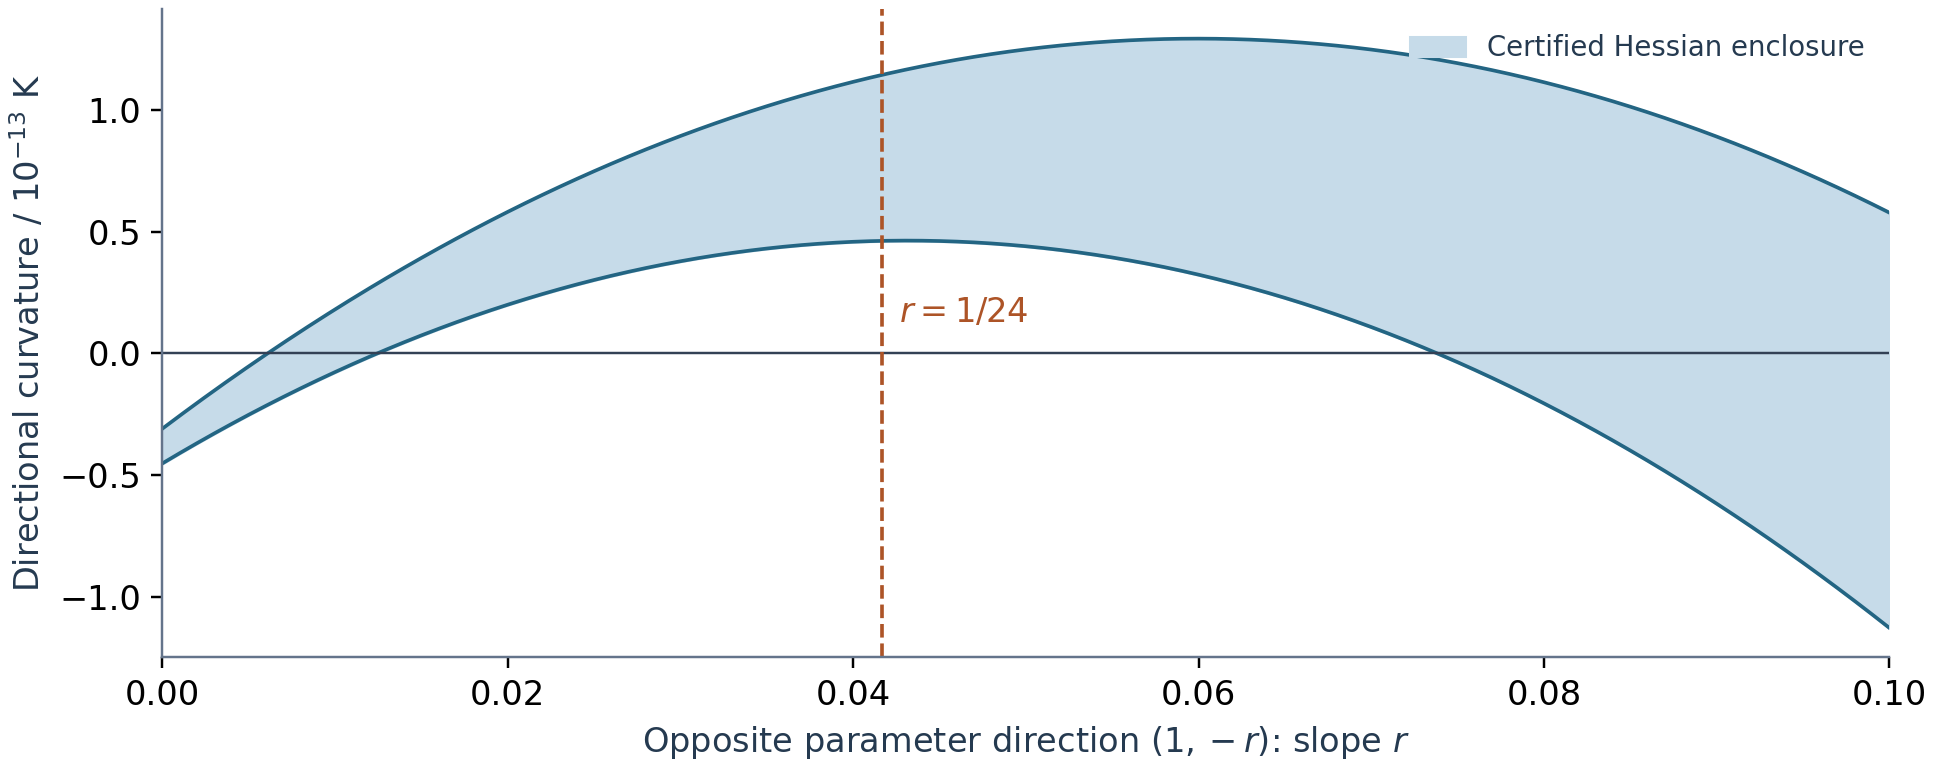
\includegraphics[width=0.95\textwidth]{figures/hessian_directions.png}
\caption{방향 $(1,-r)$의 곡률 포함. 원 유리수 포함의 decimal 표시를 이용한 시각화다.
밴드는 확률적 오차 막대가 아니라 허용 Hessian의 포함이며,
$r=1/24$의 엄격한 양성은 별도의 정확한 유리수 계산으로 판정했다.}
\end{figure}
